% Introduction

\chapter{Introduction}

\label{Introduction}
When considering a graph usually we can easily see if it is connected or not, but if it is connected what can we say about how stable or strong this connectedness is. As an example consider the following graph which might represent a computer network or something similar in applications:

\begin{figure}[ht]
\centering
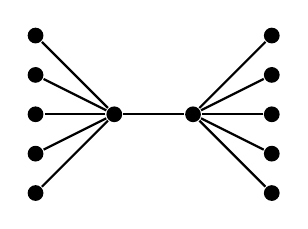
\begin{tikzpicture}[
       thick,
       acteur/.style={
         circle,
         fill=black,
         thick,
         inner sep=2pt,
         minimum size=0.2cm
       }
     ]

       \node (a1) at (0,0) [acteur]{};
       \node (a2) at (0,0.5)[acteur]{};
       \node (a3) at (0,1) [acteur]{};
       \node (a4) at (0,1.5)[acteur]{};
       \node (a5) at (0,2)[acteur]{};
       
       \node (a6) at (1,1) [acteur]{};
       \node (a7) at (2,1) [acteur]{};
       
       \node (a8) at (3,0) [acteur]{};
       \node (a9) at (3,0.5)[acteur]{};
       \node (a10) at (3,1) [acteur]{};
       \node (a11) at (3,1.5)[acteur]{};
       \node (a12) at (3,2)[acteur]{};
  
       \draw (a6) -- (a7);
       
       \draw (a7) -- (a8);
       \draw (a7) -- (a9);
       \draw (a7) -- (a10);
       \draw (a7) -- (a11);
       \draw (a7) -- (a12);
       
       \draw (a6) -- (a1);
       \draw (a6) -- (a2);
       \draw (a6) -- (a3);
       \draw (a6) -- (a4);
       \draw (a6) -- (a5);

\end{tikzpicture}
  \caption{A weakly connected graph}
  \label{figure7:Figure 7}
\end{figure}


We see that if we removed the middle edge the graph would split into two relatively large connected components, so intuitively we could say that its connectedness is not very strong. It would be helpful if we could measure the connectivity of a graph so that we can compare several graphs according to this value.\\
The classical Cheeger constant of a graph is a well-studied object and can be imagined as such a measure. Intuitively it is constructed as follows: From a connected graph we can delete edges to make it become disconnected and so there exists a smallest (in terms of numbers of vertices) connected component. Now, the Cheeger constant is the smallest quotient that can appear by deviding the number of removed edges by the size of the smallest of the resulting connected components. Formally the Cheeger constant of a graph \(G=(V,E)\) is defined by:
\[
h(G)\coloneqq \min\left\{\frac{|\delta(A)|}{|A|}A\subset V\text{, }1\leq |A|\leq\frac{|V|}{2}\right\},
\]
with \(\delta(A)\coloneqq \left\{e=(v,w)\in Ev\in A\text{, }w\in V\setminus A\right\}\).\\
\\
There is a lot of literature which studies this Cheeger constant for arbitrary graphs, whereas it is pretty easy to determine for the complete graph on \(n\)-vertices \(K_n\), where we have:
\[
h(K_n)=\left\lceil\frac{n}{2}\right\rceil
\]
This can be easily verified as follows: For any subset \(A\subset [n]\) we have
\[
\frac{|\delta(A)|}{|A|}=\frac{|A|(n-|A|)}{|A|}=n-|A|,
\]
and by the preceding definition we have \(|A|\leq\frac{n}{2}\) so we immediately get:
\[
h(K_n)=n-\left\lfloor\frac{n}{2}\right\rfloor=\left\lceil\frac{n}{2}\right\rceil
\]
A disadvantage of this Cheeger constant is that it is only defined for graphs which can only represent relations among two vertices. To measure the connectivity of constructions which can represent relations among arbitrary numbers of vertices (namely simplicial complexes) we need a more general notion of the Cheeger constant which we will study in this thesis. It was first introduced by Lineal and Meshulam (see \cite{2}) and later independently by Gromov (see \cite{3}) and is defined as follows:\\
\\
Let \(X\) be a simplicial complex. For a cochain \(\varphi\in C^k(X)\) we define the \textbf{norm} of \(\varphi\) as \(\|\varphi\|\coloneqq |\supp(\varphi)|\). Let now \(\varphi\in C^k(X)\), such that \(\|\delta^{k-1}(\phi)+\varphi\|\geq\|\varphi\|\) holds for every \(\phi\in C^{k-1}(X)\), then we call \(\varphi\) a \(k\)-\textbf{cosystole}. For general cochains \(\varphi\in C^k(X)\) we define the \textbf{cosystolic norm} of \(\varphi\) by:
\[
\|\varphi\|_{csy}\coloneqq \min\left\{\|\delta^{k-1}(\phi)+\varphi\|\phi\in C^{k-1}(X)\right\}
\]
Furthermore, any \(c\in \varphi+\im(\delta^{k-1})\) satisfying \(\|c\|=\|\varphi\|_{csy}\) is called a \textbf{cosystolic form} of \(\varphi\).\\
\\
The quotient
\[
\|\varphi\|_{exp}\coloneqq \frac{\|\delta^k(\varphi)\|}{\|\varphi\|_{csy}}
\]
is called the \textbf{coboundary expansion} of \(\varphi\) and
\[
h_k(X)\coloneqq \min_{\substack{\varphi\in C^k(X)\\\varphi\notin\im(\delta^{k-1})}}\|\varphi\|_{exp}
\]
is called the \(k\)-th \textbf{Cheeger constant} of \(X\).\\
\\
A cosystole \(\varphi\in C^k(X)\) is called a \(k\)-\textbf{Cheeger cosystole} if \(h_k(X)=\|\varphi\|_{exp}\).\\
\\
Let us study a simple example which might help to understand the preceding definitions. Consider the complete \(2\)-simplex \(\Delta^{[3]}\) and let \(\varphi\coloneqq (\{1,2\})^*\) be the cochain whose support only consists of one \(1\)-simplex. Obviously, \(\varphi\) is a cosystole since there exists no cochain \(\phi\in C^0(\Delta^{[3]})\) such that \(\delta^0(\phi)=\varphi\). Furthermore, we have \(\|\delta^1(\varphi)\|=1\) so we immediately see that \(\varphi\) is a Cheeger cosystole since we get
\[
\|\varphi\|_{exp}=\frac{\|\delta^1(\varphi)\|}{\|\varphi\|}=1,
\]
which coincides with the Cheeger constant in this case (see Equation \ref{equation1}).\\
\\
We could even define the Cheeger constants more generally for polyhedral complexes (see \cite{6}), but in this thesis we will only focus simplicial complexes.\\
Note, that the classical Cheeger constant of a graph coincides with the \(0\)-th Cheeger constant \(h_0(X)\) if we identify the cosystolic norm of a \(0\)-cochain \(\varphi\in C^0(X)\) with \(\min\left\{|\supp(\varphi)\text{, }n-|\supp(\varphi)|\right\}\), where \(n\) is the number of vertices in \(X\). For larger \(k\)'s the value of \(h_k(X)\) is not even known for all standard simplices \(X=\Delta^{[n]}\). By now we only have the estimate

\begin{equation}\label{equation1}
\frac{n}{k+2}\leq h_k(\Delta^{[n]})\leq\left\lceil\frac{n}{k+2}\right\rceil
\end{equation}

which was proven by Wallach and Meshulam (see \cite{4}, Proposition 2.1), so we have the exact value \(h_k(\Delta^{[n]})=\frac{n}{k+2}\) when \(k+2\) divides \(n\). In \cite{1} (Proposition 6.5) Kozlov showed that the upper bound is archieved when \(k=n-3\), so we have \(h_{n-3}(\Delta^{[n]})=2\) and furthermore he showed that \(h_1(\Delta^{[n]})=\frac{n}{3}\) even holds for every \(n\) which is not a power of \(2\).\\
\\
The classical \(0\)-th Cheeger constant of a graph is still pretty easy to understand intuitively, whereas the higher-dimensional generalizations raise the question what a measure of connectivity could mean in those cases. The following observation might help the reader to develop this intuition. For a graph \(G=(V,E)\) the classical Cheeger constant \(h(G)\) equals \(0\) if and only if \(G\) is disconnected, since for any non-empty proper subset of vertices \(A\subset V\), the set \(\delta(A)\) is empty, if and only if there is no edge between \(A\) and \(V\setminus A\). More generally, for a simplicial complex \(X\), the \(k\)-th Cheeger constant \(h_k(X)\) equals zero, if and only if the \(k\)-th homology group \(H_k(X)\) of \(X\) is not trivial, as follows:\\
For any cochain \(\varphi\in C^k(X)\) we have \(\|\varphi\|_{csy}>0\) if and only if \(\varphi\notin\im(\delta^{k-1})\) and \(\delta^k(\varphi)=0\) if and only if \(\varphi\in\ker(\delta^k)\), but the existence of a cochain satisfying these two properties is equivalent to \(\im(\delta^{k-1})\subsetneq\ker(\delta^k)\), which just means that \(H^k(X)\neq\{0\}\).\\
So, we have to study the Cheeger constants of those simplicial complexes whose homology vanishes and the most obvious example of those complexes is the standard simplex \(\Delta^{[n]}\).\\
\\
In the first part of this thesis we will develop some theory about the cosystolic norm of cochains, since a better understanding of cosystoles seems to be the key knowledge to determine the Cheeger constants. In the second part we will focus on the special case of \(1\)-cosystoles and the first Cheeger constant, where we have an interesting graph theoretical approach introduced by Kozlov in \cite{1}, that seems to be suited well to investigate those cosystoles in a purely combinatorial way. The last chapter adresses an interesting observation about partitioning consecutive numbers, which is not directly related to the topic of Cheeger constants, but arose during our research and might be helpful in other branches of combinatorics. At the end in the appendices we give practical algorithms including the calculation of cosystolic norms, Cheeger constants and partitionings according to the content of the last chapter.

